\documentclass{article}
\usepackage{amsmath}
\usepackage{braket}
\usepackage{amssymb}
\usepackage{hyperref}
\usepackage{booktabs}
\usepackage{graphicx}
\newcommand{\bfit}[1]{\textit{\textbf{#1}}}
\begin{document}
\textbf{\Large Chapter 6\\ Density Matrix and the Bloch Sphere}\\\\
\textbf{\large 6.1 Introduction}\\\\
In this chapter, we will first study the real vector space of 2 $\times$ 2 Hermitian matrices.
This is a vector space although its elements are matrices. We will show that any 2 $\times$ 2 Hermitian 
matrix can be represented as a linear combination of the Pauli matrices
and the identity matrix. We will then introduce the inner product of matrices,
which is just a natural extension of the concept we learned in a regular vector space.
Then we will discuss the conecpt of density matrix, which is very useful for describing
mixed states due to the lack of information or the system being entangled
with the external environment. Finally, we will show how to find the expectation values
of an operator using a density matrix. Particularly, when the operator is a linear combination of the 
Pauli matrices, its expectation value is just the projection of the state
(including mixed state) on the corresponding normalized Bloch vector on the Bloch sphere.
\\\\
\bfit{\large 6.1.1 Learning Outcomes}\\\\
Know how to perform the decomposition of a 2 $\times$ 2 Hermitian matrix into
Pauli matrices and identity matrix; know how to construct density matrices
for pure and mixed states; appreciate the meaning of the density matrix of a mixed
state and its representation on the Bloch sphere.\\\\
\bfit{\large 6.1.2 Teaching Videos}\\\\
$\bullet$ Search for Ch6 in this playlist

- \url{https://tinyurl.com/3yhze3jn}\\\\
$\bullet$ Other videos

- \url{http://youtu.be/JR2jRCeTHDc}

- \url{http://youtu.be/KEkOh9IDRI0}

- \url{http://youtu.be/4ns5_BaF4xY}

- \url{http://youtu.be/bUI5-zLR5r4}\\\\

\textbf{\large 6.2 Real Vector Space of 2 $\times$ 2 Hermitian Matrices}\\\\
In this section, we will study one special vector space, the \textbf{real vector space of} 2 $\times$ 2
\textbf{Hermitian matrices}, becuase of the following reasons. Firstly, we want to 
understand the relationship between the identity matrix and the Pauli matrices,
which is important in the equations of \textbf{density matrix}. Secondly, it reinforces
our understanding of vector space. Finally, we will take this opportunity to introduce
the concept of the \textbf{inner product of matrices}.

As the name implies, the vector space we are interested in has Hermitian matrices
as it \textit{vector elements}. A vector defining a vector space does not need to be usual 
column vector. As defined in Chap 2, a vector space is defined as long as its vectors
satisfy Eq. (2.1). The vector space should contain an addition operation and be also defined
over a set of scalar. In the real vector space of Hermitian matrices, we define the addition operation as how we perform a typical matrix
addition, and the scalars are limited to real number. Readers are encouraged to check that 
Eq. (2.1) is satisfied.

Since any of its vectors, \bfit{M}, is a 2 $\times$ 2 Hermitian matrix, then \bfit{M}=\bfit{M}$^\dagger$.
It has conly four degrees of freedom (DOFs). This is because its two diagonal elements
are real and its off-diagonal elements are complex conjugate to each other.
I/t is determined by four real numbers, $a, b, c$, and $d,$ as
\begin{equation} \label{eq 6.1}
    \boldsymbol{M}=\begin{pmatrix}
        a & b+ic\\b-ic & d
    \end{pmatrix}
    =\boldsymbol{M}^{\dagger} \tag{6.1}
\end{equation}


Therefore, this is a 4D real space (as the scalars are defined to be real). And it
turns out that its basis can be formed by the Pauli matrices and the identity matrix
which are,
\begin{align*}\label{eq 6.2}
    &\boldsymbol{I}=\boldsymbol{\sigma_0}=\begin{pmatrix}
        1 \ 0\\ 0\ 1
    \end{pmatrix},\\
    &\boldsymbol{\sigma_x}=\boldsymbol{\sigma_1}=\begin{pmatrix}
        0\ 1\\ 1\ 0
    \end{pmatrix},\\
    &\boldsymbol{\sigma_y}=\boldsymbol{\sigma_2}=\begin{pmatrix}
        0 & -i\\i&0
    \end{pmatrix},\\
    &\boldsymbol{\sigma_z}=\boldsymbol{\sigma_3}=\begin{pmatrix}
        1 &0\\ 0&-1
    \end{pmatrix}. \tag{6.2}
\end{align*}
Note that we label \bfit{I} as $\boldsymbol{\sigma_0}$. $\boldsymbol{\sigma_0}$ does not
have all the properties Pauli matrices have. For example, it is not tracelss. It does not
follow the commutation and anti-commutation relations with the Pauli matrices. But together
with the Pauli matrices, they form the basis to express any \bfit{M},
\begin{align*}\label{eq 6.3}
    \boldsymbol{M}&=\alpha_0^\prime\boldsymbol{I}+\alpha_1^\prime\boldsymbol{\sigma_x}
    +\alpha_2^\prime\boldsymbol{\sigma_y}+\alpha_3^\prime\boldsymbol{\sigma_z},\\
    &=\alpha_0^\prime\boldsymbol{\sigma_0}+\alpha_1^\prime\boldsymbol{\sigma_1}
    +\alpha_2^\prime\boldsymbol{\sigma_2}+\alpha_3^\prime\boldsymbol{\sigma_3},\\
    &=\sum_{i=1}^{3}\alpha_i^\prime\boldsymbol{\sigma_i}.\tag{6.3}
\end{align*}
Again, $\alpha_0^\prime$ to $\alpha_3^\prime$ are real based on the definition of the space.
We will also define two vectors to facilitate future derivations.
Firstly, we define a \textbf{Pauli vector} which is compsed of Pauli matrices,
\begin{equation}\label{eq 6.4}
    \boldsymbol{\vec{\sigma}}=\begin{pmatrix}
        \boldsymbol{\sigma_1}\\\boldsymbol{\sigma_2}\\ \boldsymbol{\sigma_3}
    \end{pmatrix}=
    \begin{pmatrix}
        \begin{pmatrix}
            0\ 1\\ 1\ 0
        \end{pmatrix}\\ \addlinespace
        \begin{pmatrix}
            0& -i\\i &0
        \end{pmatrix}\\ \addlinespace
        \begin{pmatrix}
            1 &0\\0&-1
        \end{pmatrix}
    \end{pmatrix}.\tag{6.4}
\end{equation}
Note that the Pauli vector is a colum vector but it has matrices as its elements!
As long as it works as a vector, why not? But note that it is not in the Hermitian
matrix space that we are discussing. It is just defined for convenience. We will also 
define a regular vector for the coefficients,
\begin{equation} \label{eq 6.5}
    \vec{\alpha^\prime}=\begin{pmatrix}
        \alpha_1^\prime\\ \alpha_2^\prime \\ \alpha_3^\prime
    \end{pmatrix}.\tag{6.5}
\end{equation}
Therefore, Eq. (\ref{eq 6.3}) may be expressed as,
\begin{align*} \label{eq 6.6}
    \boldsymbol{M}&=\sum_{i=0}^{3}\alpha_i^\prime\boldsymbol{\sigma_i},\\
    &=\alpha_0^\prime\boldsymbol{\sigma_0}+\braket{\vec{\alpha^\prime}|\vec{\boldsymbol{\sigma}}},\\
    &=\alpha_0^\prime\boldsymbol{I}+\vec{\alpha^\prime} \cdot \vec{\boldsymbol{\sigma}}.\tag{6.6}
\end{align*}
where if you perform an inner product in the second line, you will recover the first line. In the last line,
I try to rewrite it in a common (non \textit{bra-ket}) notation.\\\\
\bfit{\large 6.2.1 Trace of 2 $\times$ 2 Hermitian Matrices}\\\\
Let us now study the \textbf{trace} properties of 2 $\times$ 2 Hermitian matrices. Firstly,
\begin{align*} \label{eq 6.7}
    tr(\boldsymbol{M})&=tr(\alpha_0^\prime\boldsymbol{I})+tr(\vec{\alpha^\prime}\cdot\vec{\boldsymbol{\sigma}}),\\
    &=\alpha_0^\prime tr(\boldsymbol{I})+0=2\alpha_0^\prime.\tag{6.7}
\end{align*}
where we used the fact that the trace operation is linear and the Pauli matrices
are traceless (Eq. (5.16)). By rearranging the terms, we also find that
\begin{equation} \label{eq 6.8}
    \alpha_0^\prime=\frac{tr(\boldsymbol{M})}{2}=\frac{tr(\boldsymbol{\sigma_0M})}{2},\tag{6.8}
\end{equation}
where we have used the fact that $\sigma_0=\boldsymbol{I}$. Another property we want to know is the
trace when it is multiplied by a Pauli matrix, $\boldsymbol{\sigma_k}$, with $k=1, 2, 3$ (not including 0).
That is,
\begin{equation}\label{eq 6.9}
    tr(\boldsymbol{\sigma_kM})=tr(\alpha_0^\prime\boldsymbol{\sigma_k\sigma_0}+\alpha_1^\prime\boldsymbol{\sigma_k\sigma_1}
    +\alpha_2^\prime\boldsymbol{\sigma_k\sigma_2}+\alpha_3^\prime\boldsymbol{\sigma_k\sigma_3})\tag{6.9}
\end{equation}
This looks difficult but it is very straightforward. Since the trace operation is linear,
we can do it term by term. The first temr has a zero trace because $\boldsymbol{\sigma_0}$ 
is just the identity matrix. So the first term is just a Pauli matrix (which is traceless)
scaled by $\alpha_0^\prime$. For the other terms, they are the products of two Pauli matrices. 
Only one of them gas two identical Pauli matrices and the other two have different Pauli matrices.
For example, if $k=2,$ they become $\alpha_1^\prime\boldsymbol{\sigma_2\sigma_1}+\alpha_2^\prime\boldsymbol{\sigma_2\sigma_2}+\alpha_3^\prime\boldsymbol{\sigma_2\sigma_3}$.
Based on Eq. (5.18), the trace of the product of two different Pauli matrices is 0 and that of the same Pauli
matrices is 2. So only 2$\alpha_2^\prime$ is left. Therefore, we have
\begin{equation}\label{eq 6.10}
    tr(\boldsymbol{\sigma_kM})=2\alpha_k^\prime,\tag{6.10}
\end{equation}
and thus,
\begin{equation}\label{eq 6.11}
    \alpha_k^\prime=\frac{tr(\boldsymbol{\sigma_kM})}{2}.\tag{6.11}
\end{equation}
Combining Eqs. (\ref{eq 6.8}) and (\ref{eq 6.11}), we can write
\begin{align*} \label{eq 6.12}
    tr(\boldsymbol{\sigma_iM})&=2\alpha_i^\prime,\\
    \alpha_i^\prime&=\frac{tr(\boldsymbol{\sigma_iM})}{2},\tag{6.12    }
\end{align*}
for $i= 0, 1, 2, 3$. This is actually related to the \textit{inner product}
of the matrices which we will discuss next.\\\\
\bfit{\large 6.2.2 Inner Product of Matrices}\\\\
The real vector space of 2 $\times$ 2 Hermitian matrices is a vector space.
We can further define an \textbf{inner product} to make it an inner product space (see Chap.2).
As a reminder, the 2 $\times$ 2 Hermitian matrices are the \textit{vectors}
in this space. Therefore, the inner product must be defined over the Hermitian
matrices (which are the "vectors" in this vector space). The inner product of matrices
\bfit{A} and \bfit{B} are defined as,
\begin{equation} \label{eq 6.13}
    \braket{\boldsymbol{A|B}}=tr(\boldsymbol{A^{\dagger}B}). \tag{6.13}
\end{equation}
Therefore, the trace operator has the effect of finding the "overlap" between two
matrices. This is also called the Hilbert-Schmidt inner product or trace inner product.
It also satisfies the properties in Eq. (2.5).

Let us recall how to find the amount of a componenet in a regular vector.
Assume the vector is $\ket{\psi}=\alpha\ket{0}+\beta\ket{1}$; to find how much 
$\ket{0}$ it has, we will perform an inner product in this way,
\begin{equation}\label{eq 6.14}
    \braket{0|\psi}=\alpha\braket{0|0}+\beta\braket{0|1}=\alpha,\tag{6.14}
\end{equation}
where we used the fact that the basis vectors are orthonormal. We also note that the
\textit{bra} version of $\ket{0}$ is used. For a general Hermitian matrix, we have $\boldsymbol{M}=
\alpha_0^\prime\boldsymbol{\sigma_0}+\alpha_1^\prime\boldsymbol{\sigma_1}+
\alpha_2^\prime\boldsymbol{\sigma_2}+\alpha_3^\prime\boldsymbol{\sigma_3}$.
Therefore, we expect that we can find the amount of each componenet by using
the inner product. From Eq. (\ref{eq 6.12}), we have
\begin{align*}\label{eq 6.15}
    \alpha_i^\prime&=\frac{tr(\boldsymbol{\sigma_iM})}{2},\\
    &=\frac{tr(\boldsymbol{\sigma_i^{\dagger}M})}{2},\\
    &=\frac{\braket{\boldsymbol{\sigma_i|M}}}{2},\tag{6.15}
\end{align*}
where we have used $\boldsymbol{\sigma_i}=\boldsymbol{\sigma_i^{\dagger}}$ as they
are Hermitian. It can be seen that the amount of each componenet can be obtained by performing
an inner product and scaling it by half.\\\\
\textbf{Example 6.1} Show that $\boldsymbol{\sigma_x}$ is orthogonal to $\boldsymbol{\sigma_y}$.

We will show this by finding their inner peodcut. That is,
\begin{align*} \label{eq 6.16}
    \braket{\boldsymbol{\sigma_x|\sigma_y}}&=tr(\boldsymbol{\sigma_x^{\dagger}\sigma_y}),\\
    &=tr(\boldsymbol{\sigma_x\sigma_y}),\\
    &=0,\tag{6.16}
\end{align*} 
where we have used Eq. (5.8) in line 2 and Eq. (5.18) in line 3. Since their inner
product is zero, they are orthogonal to each other.

In general, we have (see Problem 6.5),
\begin{align*}
    \braket{\boldsymbol{\sigma_x|\sigma_y}}&=tr(\boldsymbol{\sigma_i^{\dagger}\sigma_j}),\\
    &= 2\delta_{ij}, \tag{6.17}
\end{align*}

This shows that the basis vectors, $\boldsymbol{\sigma_i}$, for $i=0,1,2,3$, are \textbf{orthogonal}
to eacth other. They are also normailzed to two (instead of one). We will not discuss its
implications. But I hope this can reinfroce our understanding of basis vectors and linear space.\\\\
\textbf{\large 6.3 Density Matrix}\\\\
\bfit{\large 6.3.1 Pure and Mixed States}\\\\
Before introducing \textbf{density matrix}, let us clarify a few important concepts regarding
quantum states in a mixture and quantum states of which we do not have complete knowledge.

Evergy quantum system must be in a certain state, $\ket{\psi}$. This is called
a \textbf{pure state}. We need to emphasize that it can be one of the basis states,
e.g., $\ket{\downarrow}$ or $\ket{\uparrow}$ in a 1-qubit system. It can also be a 
superposition state, $\alpha\ket{\downarrow}+\beta\ket{\uparrow}$. They are on the
\textbf{Bloch sphere surface}. These are all pure states (left of Fig. 6.1).\\\\
\textbf{Example 6.2} What is the probability of measureing $\ket{\downarrow}$ and $\ket{\uparrow}$ for state
$\ket{\psi}=\frac{1}{\sqrt{4}}\ket{\downarrow}+\sqrt{\frac{3}{4}}\ket{\uparrow}$?
\\\\

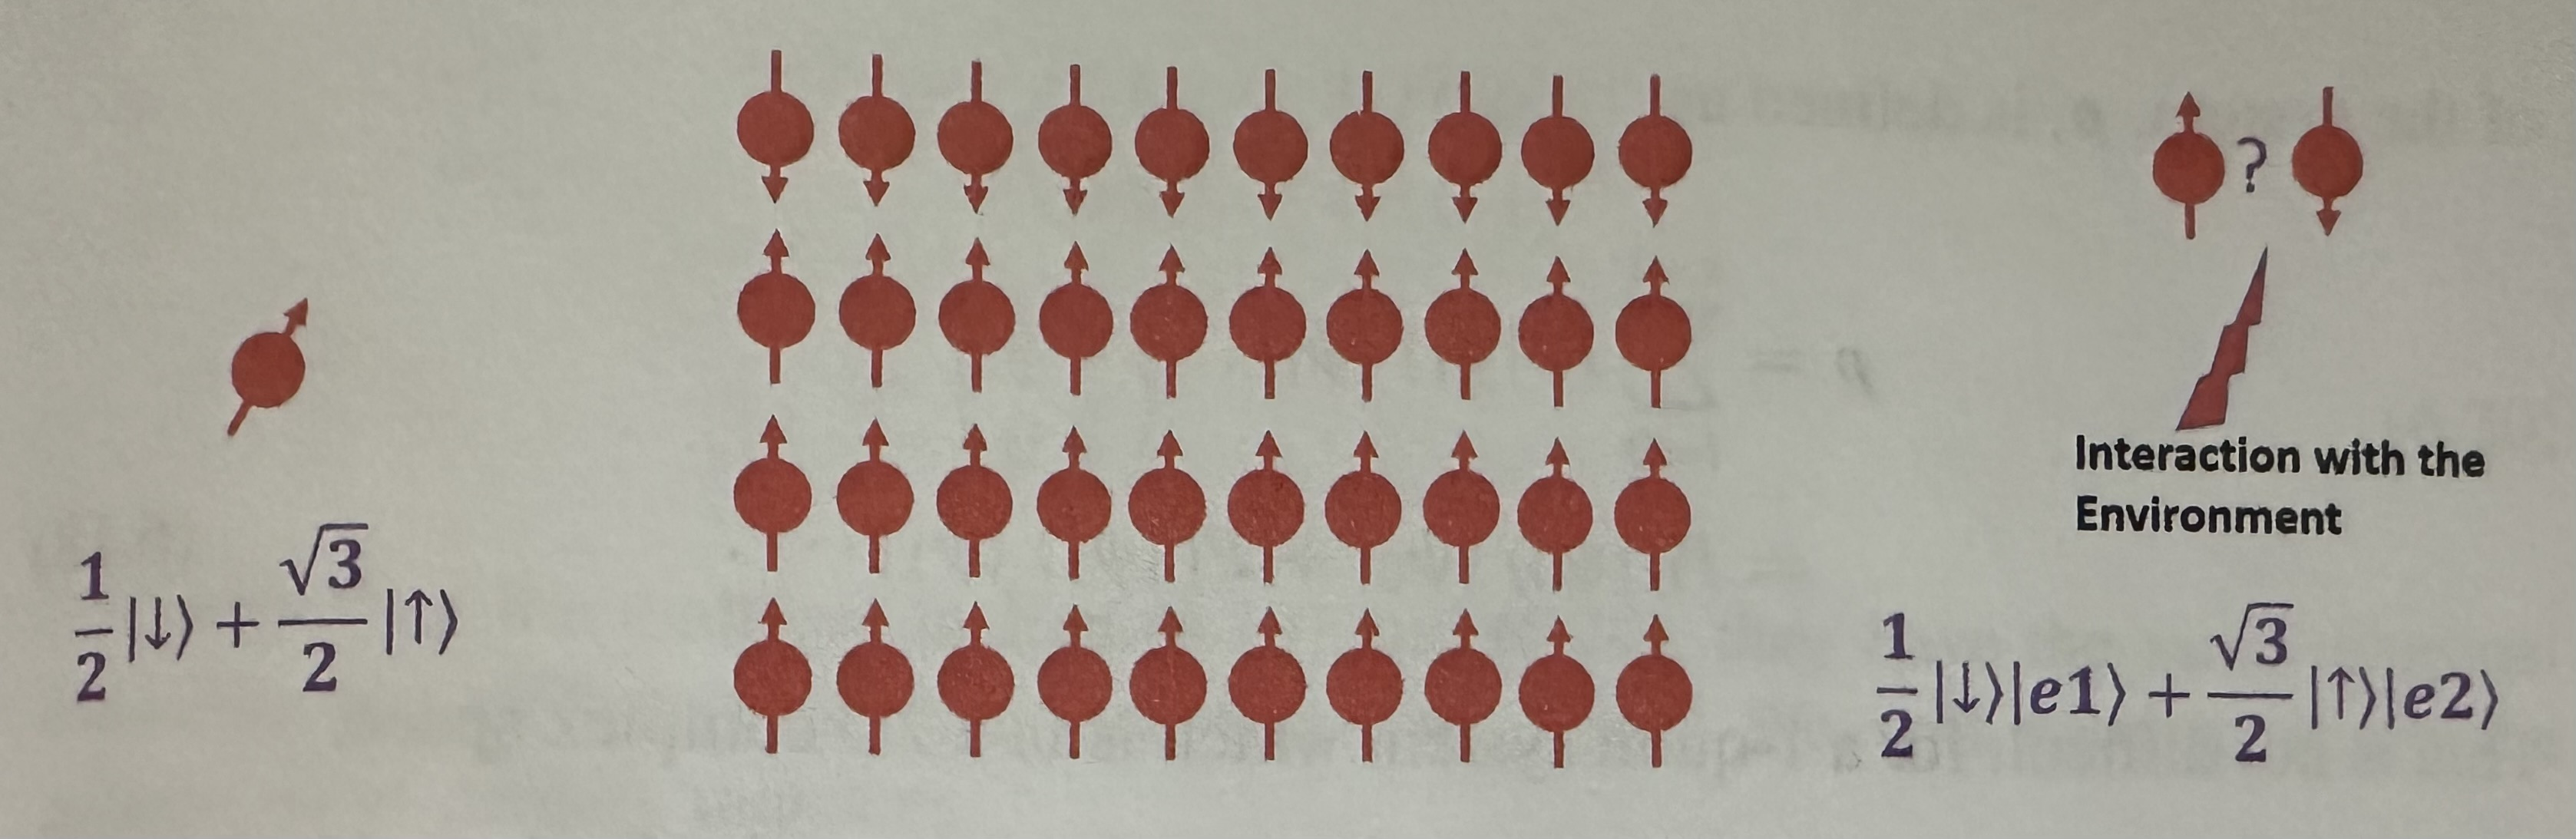
\includegraphics[scale=0.4]{Fig 6.1.jpeg}\\
\textbf{Fig. 6.1} Left: An electron in a superposition state $\frac{1}{\sqrt{4}}\ket{\downarrow}+\sqrt{\frac{3}{4}}\ket{\uparrow}$.
Middle: 40 electrons with 10 in state $\ket{\downarrow}$ and 30 in state $\ket{\uparrow}$. Right: An electron entangled with the environment
to form a pure state $\frac{1}{\sqrt{4}}\ket{\downarrow}\ket{e1}+\sqrt{\frac{3}{4}}\ket{\uparrow}\ket{e2}$. We cannot say if the electron is 
$\ket{\uparrow}$ or $\ket{\downarrow}$\\

This is a \textit{pure state}. Based on Eqs. (2.21) and (2.22). $Prob(\ket{\downarrow})=\frac{1}{4}=0.25$ and
$Prob(\ket{\downarrow})=\frac{3}{4}=0.75$.

Even though every quantum system must be in a definite state (pure state), when
the system is complex, we might not have complete information. For example, there
might be 40 or more electrons (middle of Fig. 6.1). We do not know each electrons's
exact state. But we might know statiscally, 25\% of them are $\ket{\downarrow}$ and 75\%
of them are $\ket{\uparrow}$. This is just an example. It is possible to have some of them
in a superposition state. This system is an \textbf{ensemble of pure states}. If we randomly
pick an electron and measure its state, we expect $Prob(\ket{\downarrow}) = 25\%=0.25$ and 
$Prob(\ket{uparrow})= 75\%=0.75$. While the measurement outcome statistics are the same as the pure
state, these two systems are very different.

When the quantum system (e.g., one electron) interacts with the environment, it becomes a larger
system. If we describe the larger system as a whole, it is still a 
well-defined pure state. However, if we only wnat to describe the quantum system
(i.e., the electron), then the quantum system is no longer in a pure state if
it has entangled with the environment (right of Fig.6.1). For example, the pure state
of the larger system is $\frac{1}{\sqrt{4}}\ket{\downarrow}\ket{e1}+\sqrt{\frac{3}{4}}\ket{\uparrow}\ket{e2}$,
where $\ket{e1}$ and $\ket{e2}$ are the basis states belonging to the
environment. But if we try to measure the electron spin, we still have 
$Prob(\ket{\downarrow})=\frac{1}{4}=0.25$ and $Prob(\ket{\uparrow})=\frac{3}{4}=0.75$.

The last two cases are \textbf{mixed-state} cases.\\\\
\bfit{\large 6.3.2 Density Matrix Definition}\\\\
Since we do not have complete information to describe the mixed states,
the density matrix is thus used and it can capture the essential information of the mixed
states succinctly. Assume there is a quantum system with \textit{k pure} states,
$\ket{\psi_i}$ for $i=0,1,\cdots,k-1,$ and each has a measurement probability of \textit{P}$_i$. 
The density matrix of the system, $\boldsymbol{\rho}$, is defined as,
\begin{align*} \label{eq 6.18}
    \boldsymbol{\rho}&=\sum_{i=1}^{k-1}P_i\ket{\psi_i}\bra{\psi_i},\\
    &=P_0\ket{\psi_0}\bra{\psi_0}+P_1\ket{\psi_1}\bra{\psi_1}\cdots. \tag{6.18}
\end{align*}
This is not difficult for a 1-qubit system which is in a 2D complex space.\\
\textbf{Example 6.3} Find the density matrix for the pure state and mixed state in Fig. 6.1.

For the pure state case, $\ket{\psi}=\frac{1}{\sqrt{4}}\ket{\downarrow}+\sqrt{\frac{3}{4}}\ket{\uparrow}$.
Therefore, $k=1, \ket{\psi_0}=\ket{\psi}$, and $P_0=1$. We sort the basis
vectors so that $\ket{\downarrow}$ goes first. So, $\ket{\uparrow}=\begin{pmatrix}
    1\\0
\end{pmatrix}$ and $\ket{\uparrow}=\begin{pmatrix}
    0\\1
\end{pmatrix}$. Thus,
\begin{align*} \label{eq 6.19}
    \boldsymbol{\rho}&=P_0\ket{\psi_0}\bra{\psi_0},\\
    &=1 \times \ket{\psi}\bra{\psi},\\
    &=\left( \frac{1}{\sqrt{4}}\ket{\downarrow}+\sqrt{\frac{3}{4}}\ket{\uparrow} \right) \times\left((\frac{1}{\sqrt{4}}\bra{\downarrow}+\sqrt{\frac{3}{4}}\bra{\uparrow}\right),\\
    &=\frac{1}{\sqrt{4}}\frac{1}{\sqrt{4}}\ket{\downarrow}\bra{\downarrow}+\frac{1}{\sqrt{4}}\sqrt{\frac{3}{4}}\ket{\downarrow}\bra{\uparrow}+
    \sqrt{\frac{3}{4}}\frac{1}{\sqrt{4}}\ket{\uparrow}\bra{\downarrow}+\sqrt{\frac{3}{4}}\sqrt{\frac{3}{4}}\ket{\uparrow}\bra{\uparrow},\\
    &=\frac{1}{4}\begin{pmatrix}
        1\\0
    \end{pmatrix}
    \begin{pmatrix}
    1 \ 0    
    \end{pmatrix}+
    \sqrt{\frac{3}{16}}\begin{pmatrix}
        1\\0
    \end{pmatrix}
    \begin{pmatrix}
        0 \ 1
    \end{pmatrix}+
    \sqrt{\frac{3}{16}}\begin{pmatrix}
        0\\1
    \end{pmatrix}
    \begin{pmatrix}
        1 \ 0
    \end{pmatrix}+
    \sqrt{\frac{9}{16}}\begin{pmatrix}
        0\\1
    \end{pmatrix}
    \begin{pmatrix}
        0 \ 1
    \end{pmatrix},\\
    &=\frac{1}{4}\begin{pmatrix}
        1 \ 0 \\ 0\ 0
    \end{pmatrix}
    +\frac{\sqrt{3}}{4}\begin{pmatrix}
        0 \ 1 \\ 0 \ 0
    \end{pmatrix}+
    \frac{\sqrt{3}}{4}\begin{pmatrix}
        0 \ 0 \\ 1 \ 0
    \end{pmatrix}+
    \frac{3}{4}\begin{pmatrix}
        0 \ 0 \\ 0\ 1
    \end{pmatrix},\\
    &=\begin{pmatrix}
        \frac{1}{4} & \frac{\sqrt{3}}{4}\\
        \frac{\sqrt{3}}{4} & \frac{3}{4}
    \end{pmatrix}.\tag{6.19}
\end{align*}

For the mixed-state case, we have $k=2$. And $\ket{\psi_0}=\ket{\downarrow},\ P_0=\frac{1}{4}=0.25,
\ket{\psi_1}=\ket{\uparrow},\ P_1=\frac{3}{4}=0.75$. Therefore,
\begin{align*} \label{eq 6.20}
    \boldsymbol{\rho}&=P_0\ket{\psi_0}\bra{\psi_0}+P_1\ket{\psi_1}\bra{\psi_1},\\
    &=\frac{1}{4}\ket{\downarrow}\bra{\downarrow}+\frac{3}{4}\ket{\uparrow}\ket{\uparrow},\\
    &=\frac{1}{4}\begin{pmatrix}
        1\\0
    \end{pmatrix}
    \begin{pmatrix}
        1 \ 0
    \end{pmatrix}+\frac{3}{4}
    \begin{pmatrix}
        0\\1
    \end{pmatrix}
    \begin{pmatrix}
        0 \ 1
    \end{pmatrix},\\
    &=\frac{1}{4}\begin{pmatrix}
        1 \ 0 \\ 0\ 0
    \end{pmatrix}+
    \frac{3}{4}\begin{pmatrix}
        0\ 0\\ 0\ 1
    \end{pmatrix},\\
    &=\begin{pmatrix}
        \frac{1}{4} & 0\\
        0& \frac{3}{4}
    \end{pmatrix}. \tag{6.20}
\end{align*}

Comparing the matrices in Eqs. (\ref{eq 6.19}) and (\ref{eq 6.20}), they have
the same diagonal elements but different off-diagoanl elements. Why? 
We will need to study the properties of density matrices.\\\\\\
\bfit{\large 6.3.3 Properties of Density Matrices}\\\\
If there are $m$ (e.g., 100) pure states in the mixed state, for a $N$-dimensional system,
we need $m \; N$ complex numbers to describe the system because we need $N$ complex
numbers to describe one pure state. Note that $m$ can be much larger than $N$.
With a density matrix, we only need $N^2$ numbers to describe the system.

Density matrices are \textbf{positive semi-definite (PSD)}. A PSD matrix
is Hermitian (i.e., $\boldsymbol{\rho}=\boldsymbol{\rho}^{\dagger}$) and therefore, 
density matrices are Hermitian.

A PSD matrix is defined as having all its eigenvalues, $\ket{e_i}$, being $\geq0$. This is 
equivalent to $\braket{v|\boldsymbol{\rho}|v} \geq 0$ for any vector
$\ket{v}$ (that mean the expectation value of the density matrix is
$\geq0$) or $\boldsymbol{\rho}=\boldsymbol{A}^{\dagger}\boldsymbol{A}$ which means
that it can be decomposed as the product of a matrix \bfit{A} and its adjoint.
In summary, the following are equivalent definition of PSD matrices and we can apply
them to density matrices.
\begin{align} \label{eq 6.21}
    \ket{e_i}&\geq 0,\tag{6.21}\\ 
    \braket{v|\: \boldsymbol{\rho} \: |v}&\geq0,\tag{6.22}\\ 
    \boldsymbol{\rho}=\boldsymbol{A}^{\dagger}\boldsymbol{A}. \tag{6.23}
\end{align}
Density matrices also have a trace of one. That is,
\begin{equation} \label{eq 6.24}
    tr(\boldsymbol{\rho})=1. \tag{6.24}
\end{equation}

\textbf{A matrix is a density matrix if it is PSD with a trace of one}. Indeed, the traces of the matrices in Eqs.
(\ref{eq 6.19}) and (\ref{eq 6.20}) are both one.\\\\
\textbf{Eaxmple 6.4} A mixed state contains 50\% of $\ket{0}$ and 50\% of
$\frac{1}{\sqrt{2}}(\ket{0}+\ket{1})$. Find the trace of its density matrix.

We have $k=2,\: \ket{\psi_0}=\ket{0},\: P_0=0.5,\: \ket{\psi_1}=\frac{1}{\sqrt{2}}(\ket{0}+\ket{1})$, and $P_1= 0.5$. Therefore,

\begin{align*} \label{eq 6.25}
    \boldsymbol{\rho}&=0.5\ket{0}\bra{0}+0.5\frac{1}{\sqrt{2}}(\ket{0}+\ket{1})\frac{1}{\sqrt{2}}(\ket{0}+\ket{1}),\\
    &=0.5\ket{0}\bra{0}+0.25(\ket{0}\bra{0}+\ket{0}\bra{1}+\ket{1}\bra{0}+\ket{1}\bra{1}),\\
    &=0.65\ket{0}\bra{0}+0.25\ket{0}\bra{1}+0.25\ket{1}\bra{1}+0.25\ket{1}\bra{1},\\
    &=\begin{pmatrix}
        0.75 \ 0.25\\ 0.25 \ 0.25
    \end{pmatrix}. \tag{6.25}
\end{align*}
Therefore, the trac is tr($\boldsymbol{\rho})=0.75 + 0.25 = 1$, as expected from Eq. (\ref{eq 6.24}).
\\\\\\
\bfit{\large 6.3.4 State Purity}\\\\
How do we know if a density matrix corresponds to a pure state or a mixed state?
We can used this to check,
\begin{align*}
    tr(\boldsymbol{\rho}^2)&=1 \quad \text{Pure State},\\
    tr(\boldsymbol{\rho}^2)&<1 \quad \text{Mixed State}.\tag{6.26} 
\end{align*} 
We can understand it in this way. For a pure state, we can always diagonalize it
(or choose a new basis) so that the state is one of the basis states. Then the
density matrix must be a diagonal matrix with only one non-zero element (one)
corresponding to that state. Then its square must also be diagonal with one non-zero
element (also one). That is,
\begin{equation} \label{eq 6.27}
    \boldsymbol{\rho}=\begin{pmatrix}
        0 \quad \quad \quad  \\  \ddots \quad\\\quad \quad 1 \quad\\ \quad \quad \quad \ddots
    \end{pmatrix}, \boldsymbol{\rho^2}=\begin{pmatrix}
        0 \quad \quad \quad  \\  \ddots \quad\\\quad \quad 1 \quad\\ \quad \quad \quad \ddots
    \end{pmatrix}.\tag{6.27}
\end{equation}
Therefore, $tr(\boldsymbol{\rho}^2)=1$ for a pure state. Note that the trace of a diagonalized
matrix (a transformed matrix) is the same as the trace of the matrix before diagonalization
(transformation). For mixed state, we need to go through some proof by using matrix
multiplication and Schwarz inequality. We will not do it here. However, we can consider
a simple case where all the pure states in the mixed state are orthogonal
(such as the case in Eq. (\ref{eq 6.20})). In that case, the density matrix can be diagonalized in the
basis of its pure states with the diagonal elements corresponding to the
measurement probabilites. Then the square of the density matrix is still a diagonal matrix. That is,
\begin{equation} \label{eq 6.28}
    \boldsymbol{\rho}=\begin{pmatrix}
        P_1 \quad \quad \quad  \\  \ddots \quad\\\quad \quad  \quad\\ \quad \quad \quad P_{k-1}
    \end{pmatrix}, \boldsymbol{\rho^2}=\begin{pmatrix}
        P_1^2 \quad \quad \quad  \\  \ddots \quad\\\quad \quad  \quad\\ \quad \quad \quad P_{k-1}^2
    \end{pmatrix}.\tag{6.28}
\end{equation}

Since $tr(\boldsymbol{\rho})=P_1+\cdots+P_{k-1}=1$ and the probability are all smaller
than one, the sum of their squares must be less than one. That is, $tr(\boldsymbol{\rho}^2)=
P_1^2+\cdots+P_{k-1}^2 <1$.\\\\
\textbf{Eaxmple 6.5} Show that the density matrix in Eq. (\ref{eq 6.19}) represents a pure state.

Since, 
\begin{equation} \label{eq 6.29}
    \boldsymbol{\rho}=\begin{pmatrix}
        \frac{1}{4} & \frac{\sqrt{3}}{4}\\
        \frac{\sqrt{3}}{4}& \frac{3}{4}
    \end{pmatrix}, \tag{6.29}
\end{equation}
we have,
\begin{align*} \label{eq 6.30}
    \boldsymbol{\rho}^2&=\boldsymbol{\rho}=\begin{pmatrix}
        \frac{1}{4} & \frac{\sqrt{3}}{4}\\
        \frac{\sqrt{3}}{4}& \frac{3}{4}
    \end{pmatrix}
    \begin{pmatrix}
        \frac{1}{4} & \frac{\sqrt{3}}{4}\\
        \frac{\sqrt{3}}{4}& \frac{3}{4}
    \end{pmatrix},\\
    &= \begin{pmatrix}
        \frac{1}{16}+\frac{3}{16}& \frac{\sqrt{3}}{16}+\frac{3\sqrt{3}}{16}\\
        \frac{\sqrt{3}}{16}+ \frac{3\sqrt{3}}{16}& \frac{3}{16}+\frac{9}{16}
    \end{pmatrix},\\
    &=\begin{pmatrix}
        \frac{4}{16} & \frac{4\sqrt{3}}{16}\\
        \frac{4\sqrt{3}}{16} & \frac{12}{16}
    \end{pmatrix}.\tag{6.30}
\end{align*}

Therefore, $\boldsymbol{\rho}^2=\frac{4+12}{16}=1$ and it is a pure state density matrix as expected.

\hfill $\blacksquare$
\\\\
\textbf{Example 6.6} Show the density matrix in Eq. (\ref{eq 6.20}) represents a mixed state.

Since,
\begin{equation}\label{eq 6.31}
    \boldsymbol{\rho}=\begin{pmatrix}
        \frac{1}{4} & 0\\ 0& \frac{3}{4}
    \end{pmatrix},\tag{6.31}
\end{equation}
we have,
\begin{align*} \label{eq 6.32}
    \boldsymbol{\rho}^2&=\begin{pmatrix}
        \frac{1}{4} & 0\\ 0& \frac{3}{4}
    \end{pmatrix}
    \begin{pmatrix}
        \frac{1}{4} & 0\\ 0& \frac{3}{4}
    \end{pmatrix},\\
    &=\begin{pmatrix}
        \frac{1}{16} & 0\\ 0& \frac{9}{16}
    \end{pmatrix}, \tag{6.32}
\end{align*}

Therefore, $\boldsymbol{\rho}^2=\frac{1+9}{16}< 1$ and it is a mixed-state density
matrix as expected.

\hfill $\blacksquare$\\\\
\textbf{\large 6.4 Expectation Value}\\\\
We had briefly discussed the meaning of \textbf{expectation values} in Sect. 3.4.1 and
Eq. (5.2). \textit{The expectation value of an operator \textbf{M} in the state} $\ket{v}$ is $\braket{v|\: \boldsymbol{M} \:|v}$
(by changing the symbols in Eq. 3.31). $\ket{v}$ is a pure state. \\\\
\textbf{Example 6.7} What is the expectation value of $\boldsymbol{\sigma_z}$ in state
$\ket{v}=\frac{1}{\sqrt{4}}\ket{0}+\sqrt{\frac{3}{4}}\ket{1}$?

The expectation value is,
\begin{align*} \label{eq 6.33}
    \braket{v| \: \boldsymbol{M} \:|v}&=\braket{v|\: \boldsymbol{\sigma_z} \:|v},\\
    &=\begin{pmatrix}
        \frac{1}{\sqrt{4}} \ \sqrt{\frac{3}{4}}
    \end{pmatrix}
    \begin{pmatrix}
        1 &0\\0 & -1
    \end{pmatrix}
    \begin{pmatrix}
         \frac{1}{\sqrt{4}} \\ \sqrt{\frac{3}{4}}
    \end{pmatrix},\\
    &=\begin{pmatrix}
        \frac{1}{\sqrt{4}} \ \sqrt{\frac{3}{4}}
    \end{pmatrix}
    \begin{pmatrix}
        \frac{1}{\sqrt{4}} \\ -\sqrt{\frac{3}{4}}
    \end{pmatrix},\\
    &=\frac{1}{4}-\frac{3}{4}=-\frac{2}{4}= -0.5.\tag{6.33}
\end{align*}

What if we have a mixed-state system? In principle, we can treat each pure state one by one and
then take the average.\\\\
\textbf{Eaxmple 6.8} What is the expectation value of $\boldsymbol{\sigma_z}$ in a mixed
state of $\ket{\psi_0}=\ket{0},\: P_0=\frac{1}{4}=0.25,\: \ket{\psi_1}=\ket{1}, \: P_1=\frac{3}{4}=0.75$ (same as the state in Eq. (\ref{eq 6.20}))?

Firstly, we find the expectation value of $\ket{0}$, that is, 
\begin{align*}\label{eq 6.34}
    \braket{0| \: \boldsymbol{\sigma_z} \: |0}&=\begin{pmatrix}
        1\ 0
    \end{pmatrix}
    \begin{pmatrix}
        1&0\\0&-1
    \end{pmatrix}
    \begin{pmatrix}
        1\\0
    \end{pmatrix}\\
    &=1.\tag{6.34}
\end{align*}

Similarly, the expectation value of $\ket{1}$ is -1. Therefore,
the expectation value of the mixed state is $0.25 \times 1+0.75 \times -1=-0.5$.
\hfill $\blacksquare$

Based on the meaning of expectation value and the experience we gained in
Example 6.8, if we have a mixed state with $k$ pure states, $\ket{i}$, and each has a propertion
of $p_i$, the expectation value of operator \bfit{M} is,
\begin{equation} \label{eq 6.35}
    \bra{\boldsymbol{M}}=\sum_{i=1}^{k}p_i\braket{i|\boldsymbol{M}|i}.\tag{6.35}
\end{equation}

While we are not proving it here (see Problem 6.7), it can be shown that,
\begin{align*} \label{eq 6.36}
    \braket{\boldsymbol{M}}&=\sum_{i=1}^{k}p_i\braket{i|\boldsymbol{M}|i},\\
    &=tr(\boldsymbol{M}\boldsymbol{\rho}),\\
    &=tr(\boldsymbol{\rho}\boldsymbol{M}),\\
    &=tr(\boldsymbol{\rho}^{\dagger}\boldsymbol{M}),\\
    &=\braket{\boldsymbol{\rho|\boldsymbol{M}}}, \tag{6.36}
\end{align*}
where $\boldsymbol{\rho}$ is the density matrix of the state. This shows that the expectation value of
\bfit{M} in a state with density matrix $\boldsymbol{\rho}$ is the \textit{inner product \textbf{M} and $\boldsymbol{\rho}$}.
\\\\
\textbf{Exanple 6.9} Redo Example 6.8 using Eq. (\ref{eq 6.36}).

We got the density matrix from Eq. (\ref{eq 6.20}). Therefore, the expectation value is,
\begin{align*} \label{eq 6.37}
    tr(\boldsymbol{M}\boldsymbol{\rho})&=tr(\boldsymbol{\sigma_z}\boldsymbol{\rho}),\\
    &=tr\begin{pmatrix}
        \begin{pmatrix}
            1&0\\0&-1
        \end{pmatrix} \
        \begin{pmatrix}
            \frac{1}{4} &0\\0&\frac{3}{4}
        \end{pmatrix}
    \end{pmatrix},\\
    &=tr\begin{pmatrix}
        \frac{1}{4} &0\\0&-\frac{3}{4}
    \end{pmatrix},\\
    &=-0.5. \tag{6.37}
\end{align*}

This is the same as the result in Eaxmple 6.8. \hfill $\blacksquare$\\\\\\
\textbf{\large 6.5 Density Matrix, Expectation Value, and Bloch Sphere}\\\\
Now we will discuss the relationship between a 1-qubit state density matrix, the expectation
value of Pauli matrices, and their visualization on the Bloch sphere.\\\\\\
\bfit{\large 6.5.1 Pure State Expectation Values and Projections}\\\\
In Section 27.3 in [1], we showed that, for a pure state, the expectation value of $\boldsymbol{\sigma_x}, \boldsymbol{\sigma_y}
,$ and $\boldsymbol{\sigma_z}$ in a state $\ket{\psi}$ is the projection of the state from the Bloch sphere surface
to $\hat{x},\hat{y}$ and $\hat{z}$, respectively (Fig. 6.2), where we have,
\begin{align*}\label{eq 6.38}
    \braket{\psi|\: \boldsymbol{\sigma_x} \:|\psi}&=\sin{\theta}\cos{\phi}.\tag{6.38}\\
    \braket{\psi|\: \boldsymbol{\sigma_y} \:|\psi}&=\sin{\theta}\sin{\phi}.\tag{6.39}\\
    \braket{\psi|\: \boldsymbol{\sigma_z} \:|\psi}&=\cos{\theta}.\tag{6.40}
\end{align*}

In general, the expectation value of a linear combiantion of the Pauli matrices,
$n_x\boldsymbol{\sigma_x}+n_y\boldsymbol{\sigma_y}+n_z\boldsymbol{\sigma_z}$ is,
\begin{align*} \label{eq 6.41}
    \braket{\psi|(n_x\boldsymbol{\sigma_x}+n_y\boldsymbol{\sigma_y}+n_z\boldsymbol{\sigma_z})|\psi}&=\braket{\psi|\hat{n}\cdot\vec{\boldsymbol{\sigma}}|\psi},\\
    &=n_x\sin{\theta}\cos{\phi}+n_y\sin{\theta}\sin{\phi}+n_z\cos{\theta},\\
    &=(n_x,n_y,n_z)\begin{pmatrix}
        \sin{\theta}\cos{\phi}\\
        \sin{\theta}\sin{\phi}\\
        \cos{\theta}
    \end{pmatrix},\\
    &=\hat{n}\cdot\vec{\psi}. \tag{6.41}
\end{align*}
where $\hat{n}\cdot\vec{\psi}$ is just the proejction of $\vec{\psi}$ on $\hat{n}$ or their inner product.
In line 1, we used the definition of the Pauli vector, $\vec{\boldsymbol{\sigma}}$, in Eq. (\ref{eq 6.4}). 
We have used Eq. (\ref{eq 6.38}) to (6.40) in line 2 and the linear property of
\textit{bra-ket} operation. We also defined a unit directional vector, $\hat{n}$, with
\begin{equation}\label{eq 6.42}
    \hat{n}=\begin{pmatrix}
        n_x\\n_y\\n_z
    \end{pmatrix} \tag{6.42}
\end{equation}
and vector $\vec{\psi}$, which is the real space vector in the real 3D space pointing at the
location where $\ket{\psi}$ resides on the embedded Bloch sphere (Fig. 6.2) That is, 
\\

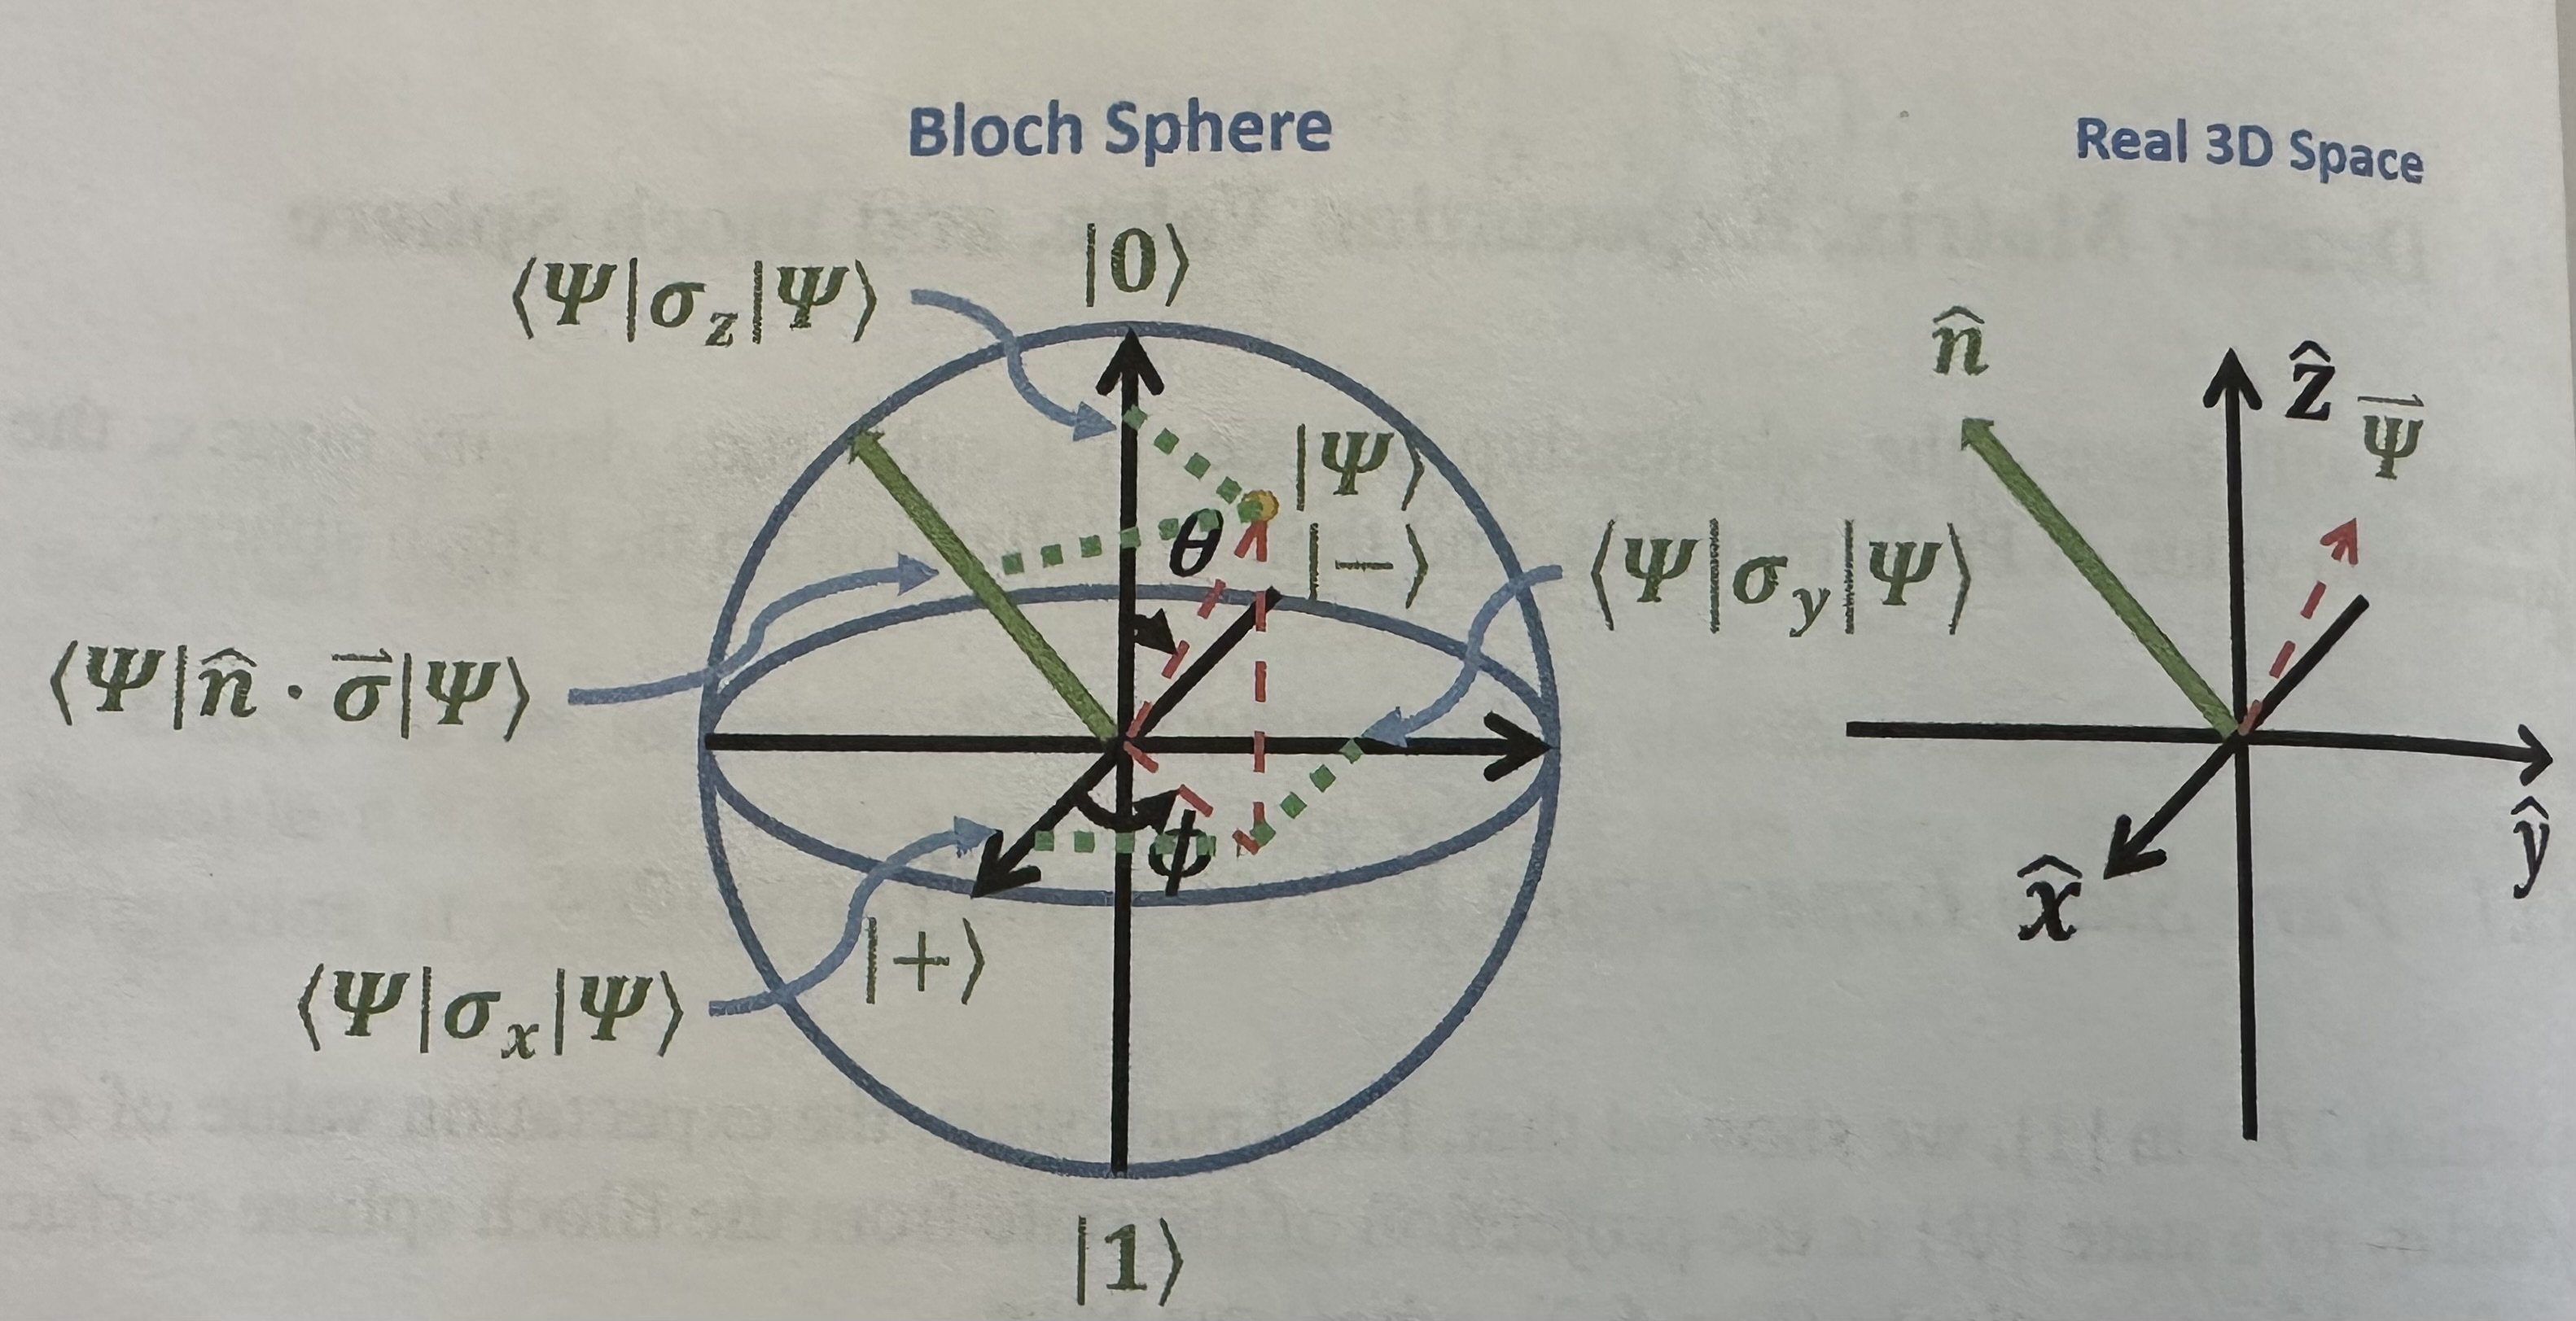
\includegraphics[scale=0.4]{Fig. 6.2.jpeg}\\
\textbf{Fig. 6.2} Left: Bloch sphere showing that the expectation values of the Pauli matrices are just the
projectinos of the state on the axes. It also shows that the expectation value of $\hat{n}\cdot\vec{boldsymbol{\sigma}}$ is the
projection on $\hat{n}$. Right: The real 3D space coordinate system with $\vec{\psi}$ and $\hat{n}$ shown.
\begin{equation}\label{eq 6.43}
    \vec{\psi}=\begin{pmatrix}
        \sin{\theta}\cos{\phi}\\
        \sin{\theta}\sin{\phi}\\
        \cos{\theta}
    \end{pmatrix}\tag{6.43}
\end{equation}

It should be noted that the radius of the Bloch sphere is one and the lengths
of $\hat{n}$ and $\vec{\psi}$ are also one. In summary, \textit{the expectation value of 
$\hat{n}\cdot\vec{\boldsymbol{\sigma}}$ is just the projection of $\psi$ and $\hat{n}$}
in our real 3D space (Fig. 6.2).\\\\\\
\bfit{\large 6.5.2 Density Matrix of a 1-Qubit System}\\\\
As dicussed earlier, a density matrix is Hermitian. A 2 $\times$ 2 Hermitian
matrix only has 4 DOFs (Eq. (\ref{eq 6.1})). Therefore, it can be decomposed as a linear
combination of four orthogonal basis vectors (note that, here, vector means the vector in a
linear space whtich is a 2 $\times$ 2 Hermitian matrix; see Sect. 6.2) with
four real coefficients. Therefore, it belongs to the real vector space of 2 $\times$ 2
Hermitian matrices. As a result, it can be decomposed in the form of Eq. (\ref{eq 6.6}),
\begin{align*}\label{eq 6.44}
    \boldsymbol{\rho}&=a_0^\prime\boldsymbol{I}+\vec{a^\prime}\cdot\vec{\boldsymbol{\sigma}},\\
    &=a_0^\prime\boldsymbol{I}+a_1^\prime\boldsymbol{\sigma_x}+
    a_2^\prime\boldsymbol{\sigma_y}+a_3^\prime\boldsymbol{\sigma_z}.\tag{6.44}
\end{align*}

We now introduce new variables,
\begin{align*}\label{eq 6.45}
    a_0&=2a_0^\prime,\tag{6.45}\\
    \vec{a}&=2\vec{a^\prime},\tag{6.46}
\end{align*}
where $\vec{a}$ is the \textbf{Bloch vector}. Then,
\begin{equation}\label{eq 6.47}
    \boldsymbol{\rho}=\frac{a_0\boldsymbol{I}+\vec{a}\cdot\vec{\boldsymbol{\sigma}}}{2}.\tag{6.47}
\end{equation}

We can further simplify it. Based on Eq. (\ref{eq 6.24}) in the last
line for a density matrix. Therefore,
\begin{equation}\label{eq 6.49}
    \boldsymbol{\rho}=\frac{\boldsymbol{I}+\vec{a}\cdot\vec{\boldsymbol{\sigma}}}{2}.\tag{6.49}
\end{equation}

Let us study the meaning of the Bloch vector, $\vec{a}$. We will first look at the matrix components
of $\boldsymbol{\rho}^2$. $\boldsymbol{\rho}$ in its matrix form is,
\begin{align*}\label{eq 6.50}
    \boldsymbol{\rho}&=\frac{1}{2}\left(\begin{pmatrix}
        1\ 0\\ 0\ 1
    \end{pmatrix}+a_x\begin{pmatrix}
        0\ 1\\ 1\ 0
    \end{pmatrix}
    +a_y\begin{pmatrix}
        0&-i\\i&0
    \end{pmatrix}
    +a_z\begin{pmatrix}
        1&0\\0&-1
    \end{pmatrix}\right),\\
    &=\frac{1}{2}\left(\begin{pmatrix}
        1\ 0\\ 0\ 1
    \end{pmatrix}+\begin{pmatrix}
        0&a_x\\a_x&0
    \end{pmatrix}+
    \begin{pmatrix}
        0& -ia_y\\ia_y&0
    \end{pmatrix}+
    \begin{pmatrix}
        a_z&0\\0&-a_z
    \end{pmatrix}\right),\\
    &=\frac{1}{2}\begin{pmatrix}
        1+a_z&a_x+ia_y\\
        a_x+ia_y&1-a_z
    \end{pmatrix}.\tag{6.50}
\end{align*}
Then,
\begin{align*} \label{eq 6.51}
    \boldsymbol{\rho}^2&=\frac{1}{2}\begin{pmatrix}
        1+a_z & a_x-ia_y\\a_x+ia_y&1-a_z
    \end{pmatrix}
    \frac{1}{2}\begin{pmatrix}
        1+a_z&a_x-ia_y\\
        a_x+ia_y&1-a_z
    \end{pmatrix},\\
    &=\frac{1}{4}\begin{pmatrix}
        a_x^2+a_y^2+a_z^2+2a_z+1&2(a_x-ia_y)\\
        2(a_x+ia_y)&a_x^2+a_y^2+a_z^2-2a_Z+1
    \end{pmatrix} \tag{6.51}
\end{align*}
Therefore,
\begin{align*}\label{eq 6.52}
    tr(\boldsymbol{\rho}^2)&=\frac{1}{4}(a_x^2+a_y^2+a_x^2+2a_z+1+a_x^2+a_y^2+a_z^2-2a_z+1),\\
    &=\frac{a_x^2+a_y^2+a_z^2+1}{2},
    &=\frac{|\vec{a}|^2+1}{2}.\tag{6.52}
\end{align*}

Based on Eq. (6.26), $tr(\boldsymbol{\rho}^2)=1$ \textit{for pure state; therefore,} $|\vec{a}|=1$. 
\textit{If it is a mixed state}, $tr(\boldsymbol{\rho}^2)<1$ \textit{and therefore},
$|\vec{a}|<1$.

To further understand the meaning of $\vec{a}$, let us consider the
expectation value of $\hat{n_a}\cdot\vec{\boldsymbol{\sigma}}$ in the
state which gives the density matrix $\boldsymbol{\rho}=\frac{I+\vec{a}\cdot\vec{\boldsymbol{\sigma}}}{2}$.
Since $\vec{a}$ can be smaller than one, we normalize it to 
$\hat{n_a}=\frac{\vec{a}}{|\vec{a}|}$ in the observable (Fig. 6.3).

This has the same form as the one in Eq. (\ref{eq 6.41}), except that now
$\hat{n}$ is $\hat{n_a}$, which is the unit vector along the direction of $\vec{a}$.
We will use the expectation value equation in Eq. (\ref{eq 6.36}) using the given density matrix,
\begin{align*}\label{eq 6.53}
    \braket{\hat{n_a}\cdot\vec{\boldsymbol{\sigma}}}&=tr(\hat{n_a}\cdot\vec{\boldsymbol{\sigma}}\boldsymbol{\rho}),\\
    &=tr(\hat{n_a}\cdot\vec{\boldsymbol{\sigma}}\frac{\boldsymbol{I}+\vec{a}\cdot\vec{\boldsymbol{\sigma}}}{2}),\\
    &=\frac{1}{2|\vec{a}|}tr(\vec{a}\cdot\vec{\boldsymbol{\sigma}}+\vec{a}\cdot\vec{\boldsymbol{\sigma}}\vec{a}\cdot\vec{\boldsymbol{\sigma}}),\\
    &=\frac{1}{2|\vec{a}|}tr(\vec{a}\cdot\vec{\boldsymbol{\sigma}}\vec{a}\cdot\vec{\boldsymbol{\sigma}}),\\
    &=\frac{1}{|\vec{a}|}(a_x^2+a_y^2+a_z^2),\\
    &=\frac{|\vec{a}|^2}{|\vec{a}|},\\
    &=|\vec{a}|. \tag{6.53}
\end{align*}
From line 3 to line 4, we have used the fact that the Pauli matrices are traceless,
and therefore, $tr(\vec{a}\cdot\vec{\boldsymbol{\sigma}})=0$ (Eq. (5.16)). In line 4, 
the squared term, $(\vec{a}\cdot\vec{\boldsymbol{\sigma}})^2$, gives rise to terms
in the form of $a_la_m\boldsymbol{\sigma_l}\boldsymbol{\sigma_m}$. One type is like
$a_xa_x\boldsymbol{\sigma_x}\boldsymbol{\sigma_x}$ which has a trace of $2a_x^2$.
Another type are cross-terms like $a_xa_y\boldsymbol{\sigma_x}\boldsymbol{\sigma_y}$ which
has a trace of 0 (see Eq. (5.18)). Therefore, only $2(a_x^2+a_y^2+a_z^2)$ is left after taking
the trace.

The result in Eq. (\ref{eq 6.53}) tells us that the expectation value of 
$\hat{n_a}\cdot\vec{\boldsymbol{\sigma}}$ in the state $\boldsymbol{\rho}=\frac{I+\vec{a}\cdot\vec{\boldsymbol{\sigma}}}{2}$
is $|\vec{a}|$.

If $|\vec{a}|=1$, we know that this density matrix correspond to a pure state $\ket{\psi}$
(Eq. (\ref{eq 6.52})). We also know that the expectation value in Eq. (\ref{eq 6.53}) is just
the inner product of $\vec{\Psi}$ and $\vec{a}$ (Sect. 6.5.1 and Eq. (\ref{eq 6.41})).
Since the inner product is one, it means that $\vec{\Psi}=\vec{a}$ and this density matrix corresponds
to a pure state that resides on the surface of the Bloch sphere at $\vec{a}$ (left of Fig. 6.3). Therefore,
the Bloch vector of a pure state is just the location of that state on the Bloch sphere.

If $|\vec{a}|<1$, it corresponds to a mixed state (right of Fig. 6.3). Since a mixed-state
density matrix is not uniquely mapped to a mixture of pure states,
we cannot deduce which mixture it is. One of the possible mixtures is having a pure
state at $\hat{n_a}$ with a

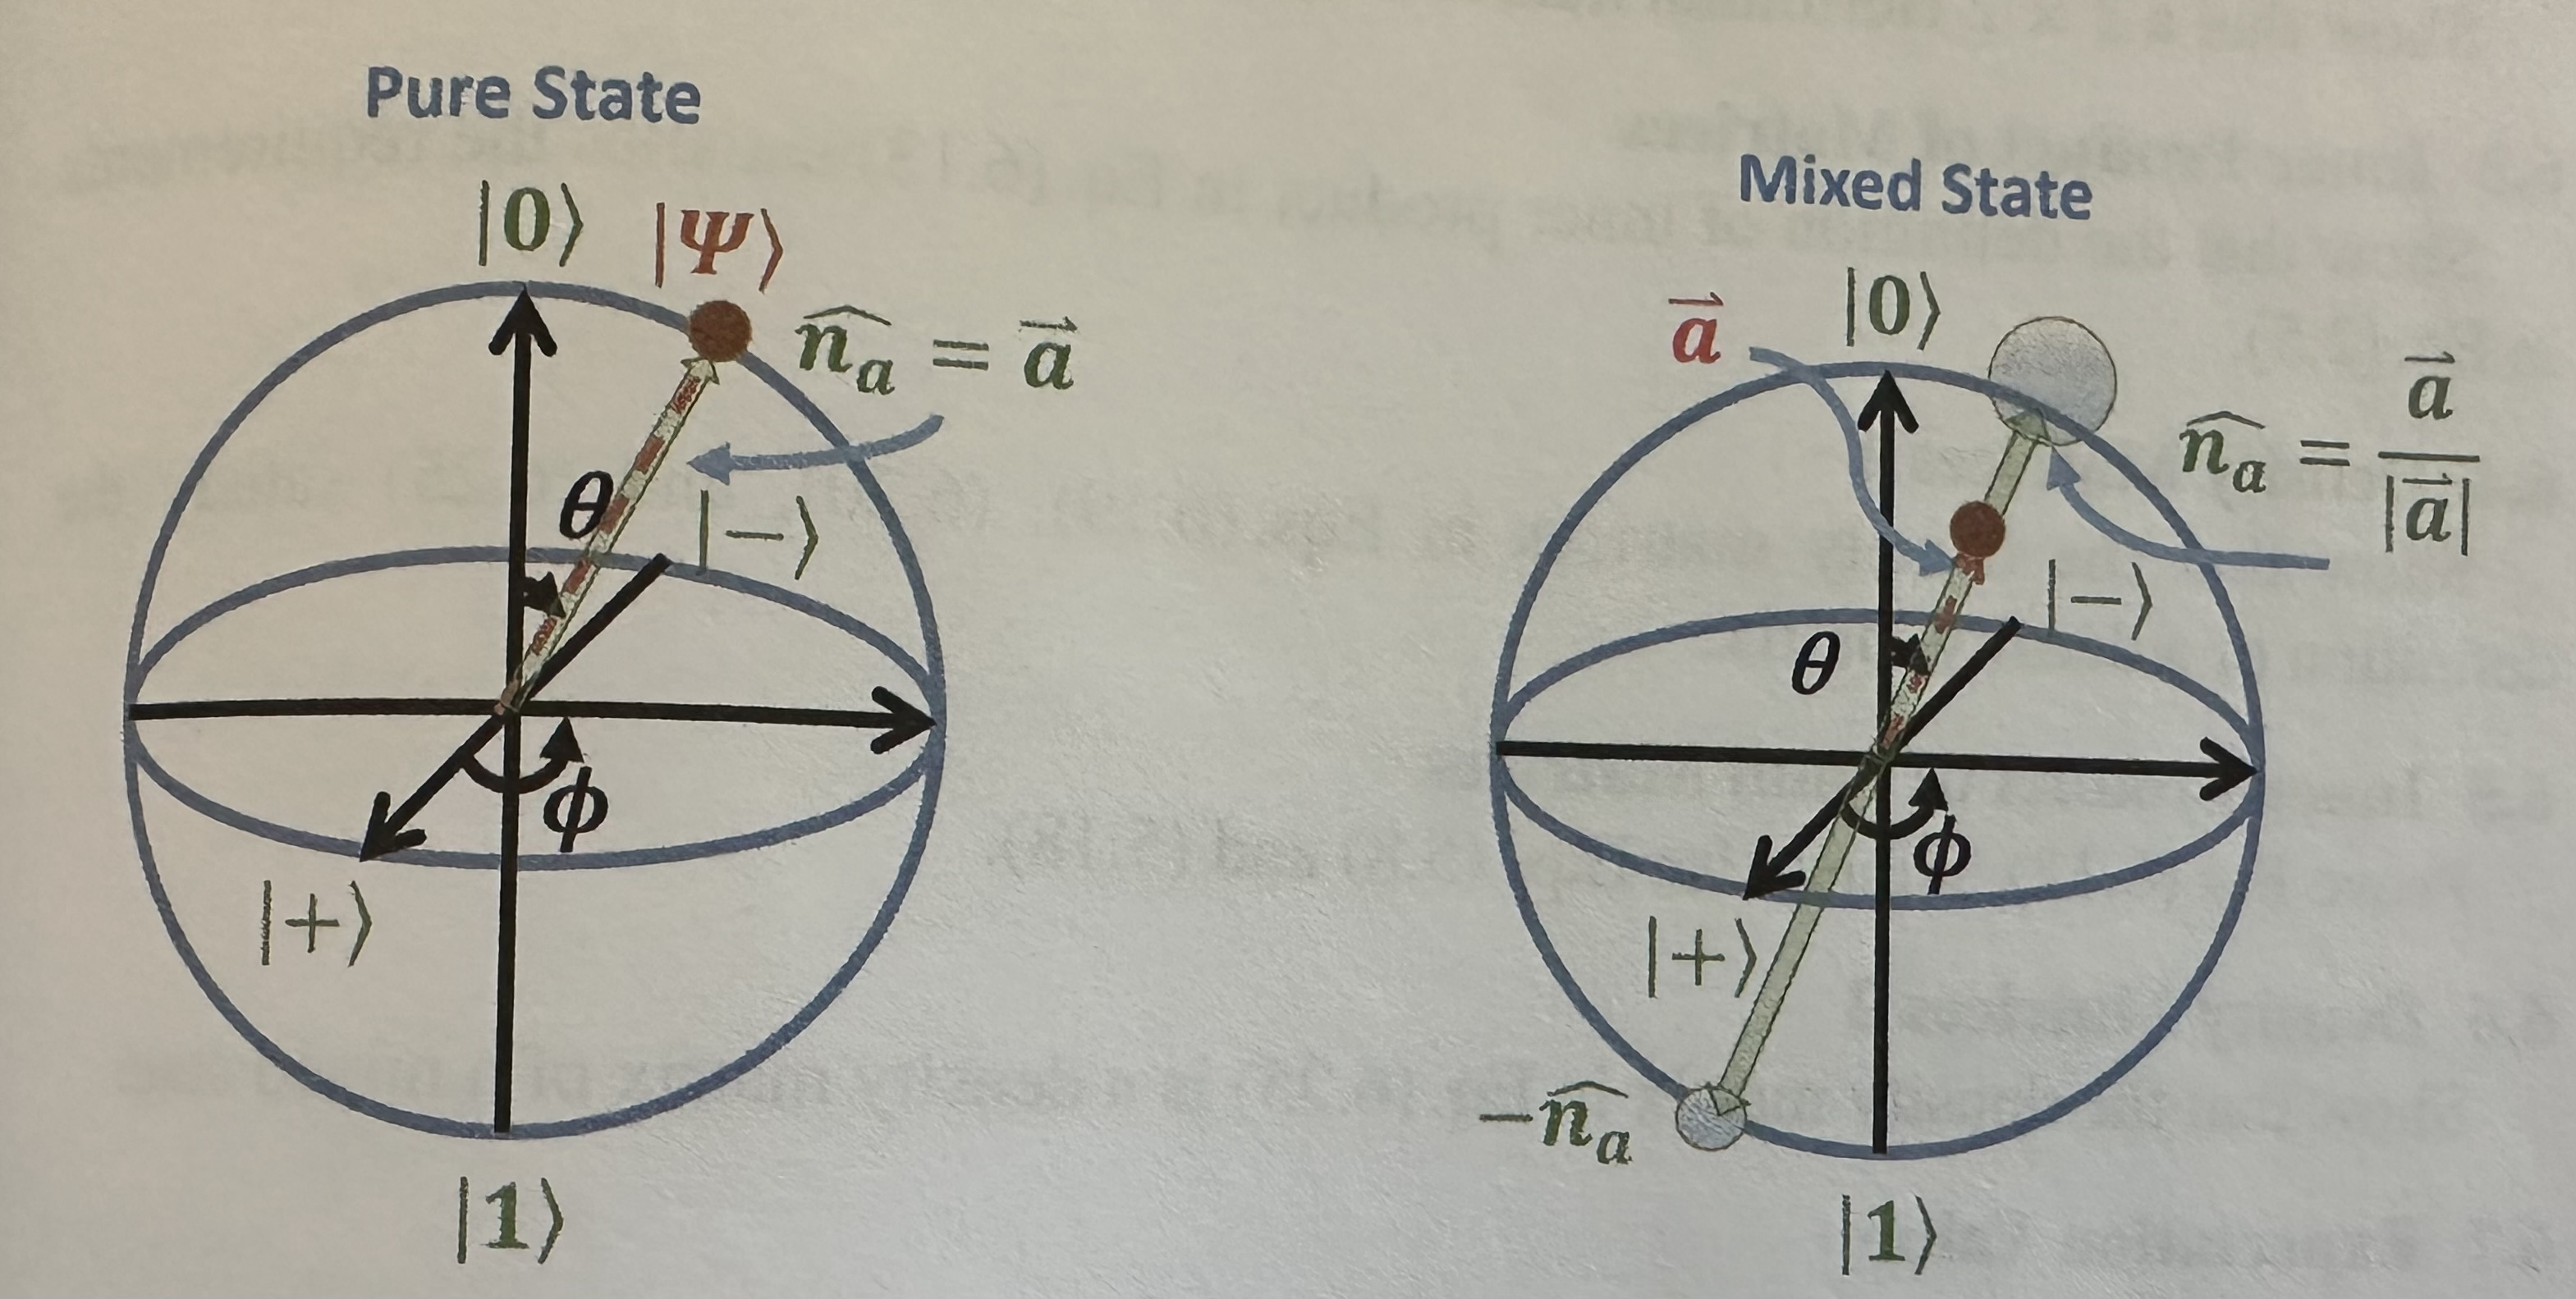
\includegraphics[scale=0.4]{Fig 6.3.jpeg}
\\\\
\textbf{Fig. 6.3} Left: Bloch sphere with the Bloch vector $\vec{a}$ shown. 
Density matrix  $\boldsymbol{\rho}=\frac{I+\vec{a}\cdot\vec{\boldsymbol{\sigma}}}{2}$ 
corresponds to a pure state $\ket{\psi}$ on the surface of the Bloch sphere residing at
$\hat{n_a}=\vec{a}$. Therefore, $\vec{a}$ is a unit vector for a pure state. Right: When the 
density matrix is of a mixed state, $\vec{a}$ is smaller than 1 and resides inside the Bloch sphere\\\\
probability of $P_0$ and a pure state at $-\hat{n_a}$ with a probability of 
$P_1$, with $P_0-P_1=|\vec{a}|$ and $P_0+P_1=1$ (readers are encouraged to prove this and 
find out what happens if $P_0=P_1$). We may say that the mixed state is represented by a point 
\textit{inside} the Bloch sphere.\\\\\\
\textbf{\large 6.6 Summary}\\\\
In this chapter, wepractice the mathematics of a more advanced linear space
that has matrices as its elements. The elements are 2 $\times$ 2 Hermitian matrices.
They can be decomposed into the linear ocmbination of the Pauli matrices and the 
identity matrix. Density matrices, which are elements of this space, are convenient representations
for mixed states. We study the properties of density matrices. We also study its representation on the
Bloch sphere. The most important conclusion is that when the state is a mixed state,
it is represented as a point inside the Bloch sphere.\\\\\\
\textbf{Problems}\\\\
\textbf{6.1 Real Vector Space of Hermitian Matrices}

Show it satisfied Eq. (2.1). What are the 1 and $\vec{0}$ in this space?\\\\
\textbf{6.2 Hermitian Matrices}

Show that 2 $\times$ 2 Hermitian matrix only has 4 DOFs instead of 8 DOFs.\\\\
\textbf{6.3 Inner Product of Matrices}

Show that the definition of inner product in Eq. (\ref{eq 6.13}) satisfies
the requirements in Eq. (2.5).\\\\
\textbf{6.4 Density Matrices 1}

Show that the density matrices in Eqs.(\ref{eq 6.19}), (\ref{eq 6.20}), and
(\ref{eq 6.25}) satisfy the definition of a density matrix.\\\\
\textbf{6.5 Inner Product of Pauli Matrices}

Prove Eq. (6.17). Hints" Use Eqs. (5.8) and (5.18).\\\\
\textbf{6.6 Density Matrices 2}

Show that the density matrix in Eq. (\ref{eq 6.25}) is a density matrix of a mixed state.\\\\
\textbf{6.7 Expectation Value}

Prove Eq. (\ref{eq 6.36}).\\\\
\textbf{6.8 Expectation Value 2}

Prove Eq. (\ref{eq 6.38}) to (6.40).\\\\\\
\textbf{\large Reference}\\\\
1. Hiu-Yung Wang. \textit{Introduction in Quantum Computing}. Springer, 2024.
\end{document}